\subsection{Критическая интенсивность}

    Критической интенсивностью называется такое значение интенсивности, при котором траектории могут выходить за границы аттрактора и сваливаться в ноль.

    Например, на рисунке \ref{critical_intensity_beta_noise} изображен график критической интенсивности для \(\beta\)-шума. Красным показана критическая интенсивность для границ доверительных интервалов, которые лежат ниже устойчивого равновесия. Синим - для границ, которые выше устойчивого равновесия. 

    \comment{Для 4-цикла сделать шаг меньше и подойти ближе к 2-циклу. Холмик должен получится}

    \begin{figure}
        \centering
        \subfloat[Модель (\ref{beta_chaos})]{
            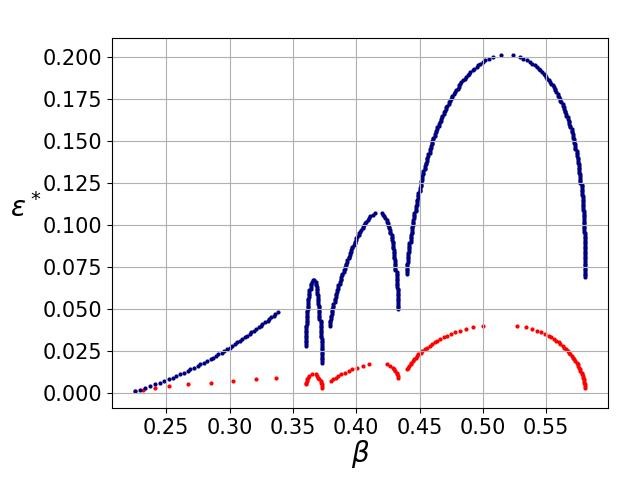
\includegraphics[width=0.55\textwidth]{stochastic/images/critical_intensity_beta_noise.jpg}
            \label{critical_intensity_beta_noise}
        }  

        \subfloat[Модель (\ref{alpha_chaos})]{
            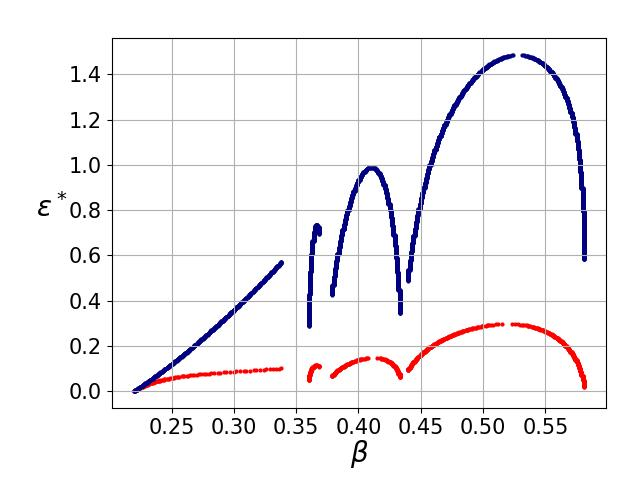
\includegraphics[width=0.55\textwidth]{stochastic/images/critical_intensity_alpha_noise.jpg}
            \label{critical_intensity_alpha_noise}
        }
        
        \subfloat[Модель (\ref{additive_chaos})]{
            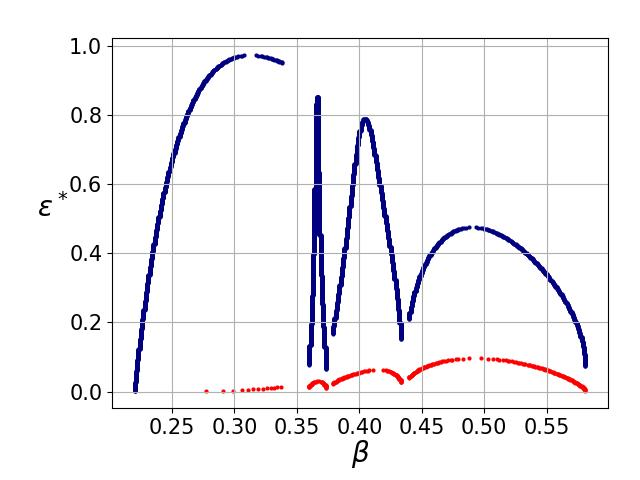
\includegraphics[width=0.55\textwidth]{stochastic/images/critical_intensity_additive_noise.jpg}
            \label{critical_intensity_additive_noise}
        }
            
        \caption{Критическая интенсивность}
    \end{figure}
    
    Обозначения аналогичны для графиков \(\alpha\)-шума (\ref{critical_intensity_alpha_noise}) и аддитивного шума (\ref{critical_intensity_additive_noise}).

    Интересно заметить, что в случае \(\alpha\)-шума и \(\beta\)-шума силуэты графиков очень похожи. В то же время график для аддитивного шума не похож на предыдущие случаи.
